\chapter{Wprowadzenie}

Szblon ten jest propozycją składu pracy dyplomowej inżynierskiej lub
magisterskiej. Poniżej znajdują się przykłady pozwalające na
szybkie zapoznanie się z podstawowymi elementami dokumentu takimi jak
tablice, rysunki, wyliczenia itp.

Przed oddaniem tego dokumentu prawidłowo wypełnić jego początkowe strony
tj.:
\begin{itemize}
\item stronę tytułową: rocznik, typ (magisterska/inżynierska),
imię i~nazwisko autora, tytuł, imię i~ nazwisko promotora pracy,
\item życiorys: data urodzenia, datę rozpoczęcia studiów, zdjęcie i~
życiorys autora,
\item streszczenie oraz słowa kluczowe w~języku polskim i~angielskim.
\end{itemize}

Szczegółowe opcje klasy {\tt mwrep}, którą wykorzystuje ten dokument,
opisane są w~dokumentacji.

\section[Tytuł w paginie][Tytuł w spisie treści]{Przykład pierwszy}

Pozostałe pliki (w głównej gałęzi katalogu 5015) reprezentują logikę struktury
PKCS~\#15 oraz certyfikaty (pliki 4545, 4546, 4547). Jej szczegółowy
opis zamieszczono w~\cite[130-140]{bk:ipki}. W~
tablicy \ref{tab:card} zebrano podstawowe dane o~wszystkich plikach.
Rozmiar niektórych plików może być różny dla innych danych wejściowych.
Dotyczy to w~szczególności certyfikatów.

Należy przyjąć, że aplikacja PKCS~\#15 w~karcie zajmuje do 6kB. W~karcie
{\it Cryptoflex 32K} pozsostaje więc około 26 kB możliwych do wykorzystania
przez inne aplikacje. W~szczególności mogą to być kolejne aplikacje PKCS~\#15
o~innym profilu zastosowań.

\begin{table}
\centering
\caption{Wykaz plików karty {\it Cryptoflex 32K} z~aplikacją PKCS~\#15}
\label{tab:card}
\begin{minipage}{.9\textwidth}
\setlength{\baselineskip}{2mm}
\centering
\begin{tabular}{c|c|c|c}
FID\footnote{ang. {\em file identifier} -- identyfikator pliku} & Rozmiar\footnote{rozmiar plików zawierających certyfikaty może być inny (w zależności od umieszczonego certyfikatu)} & Rodzaj pliku & Podstawowe prawa\\
 & (w bajtach) & & dostępu\footnote{stosowane oznaczenia: R~(ang. {\em read}) -- odczyt, U~(ang. {\em update}) -- zmiana, C~-- operacje kryptograficzne, NEV (ang. {\em never}) -- nigdy, CHV1 (ang. {\em cardholder verification}) -- kod uwierzytelniający użytkownika, ALW (ang. {\em always}) -- zawsze, AUT (ang. {\em authenticate}) -- uwierzytelnienie z~użyciem klucza}\\ \hline
3F00		    & --		   & DF\footnote{ang. {\em dedicated file} -- plik dedykoway, katalog}	& -- \\ \hline
0011		    & 27		   & EF\footnote{ang. {\em elementary file} -- plik elementarny}	& R: NEV, U: AUT \\ \hline
0002		    & 8			   & EF, TR\footnote{ang. {\em transparent} -- struktura transparentna, przeźroczysta} & R: ALW, U: NEV \\ \hline
5015		    & --		   & DF		    & -- \\ \hline
4401\footnote{identyfikatory podano bez pełnych ścieżek, zobacz rysunek \ref{ppkcs15fs}}	    & 255		   & EF, TR		    & R: ALW, U: AUT \\ \hline
4402		    & 255		   & EF, TR		    & R: ALW, U: AUT \\ \hline
5031		    & 255		   & EF, TR		    & R: ALW, U: AUT \\ \hline
5032		    & 33		   & EF, TR		    & R: ALW, U: AUT \\ \hline
4545		    & 849		   & EF, TR		    & R: ALW, U: AUT \\ \hline
4546		    & 847		   & EF, TR		    & R: ALW, U: AUT \\ \hline
4547		    & 849		   & EF, TR		    & R: ALW, U: AUT \\ \hline
4946		    & 127		   & EF, TR		    & R: ALW, U: AUT \\ \hline
4B01, 4B02	    & --		   & DF		    & -- \\ \hline
0000		    & 16		   & EF, CHV\footnote{ang. {\em cardholder verification} -- kody służące do uwierzytelnienia użytkownika} & R: NEV, U: CHV1 | AUT \\ \hline
3045, 3047	    & --		   & DF		    & -- \\ \hline
0012		    & 326		   & EF, PRVK\footnote{ang. {\em private key} -- klucz prywatny} & R: NEV, U: AUT, C: CHV1 \\ \hline
1012		    & 330		   & EF, PUBK\footnote{ang. {\em public key} -- klucz publiczny} & R: ALW, U: AUT, C: ALW \\ \hline
2F00		    & 127		   & EF, TR		    & R: ALW, U: AUT \\
\end{tabular}
\end{minipage}
\end{table}

\subsubsection{Założenia}
Dany jest zbiór pewnych maszyn. Każda z~nich charakteryzuje się pewnym
typem i~lokalizacją. Maszyny złożone są z~pewnych modułów.

Każda z~maszyn raportuje do systemu centralnego zdarzenia jakie na niej
zachodzą. Należą one do jednej z~kategorii:
\begin{itemize}
\item normalne zdarzenie
\item błąd -- zdarzenie to zawiera opis zgłaszanego błędu (moduł);
wyróżniamy błędy krytyczne (maszyna nie działa) i~ostrzeżenia (np. brakuje
zasobów dla pewnego modułu)
\item interwencja -- o~kategorii lokalnej (np. maszyna sama się naprawiła)
lub zdalnej (wymagana interwencja człowieka)
\end{itemize}

Na maszynach zachodzą pewne transakcje, których przebieg raportowany jest w~
postaci normalnych zdarzeń (chyba, że w~trakcie pojawi się błąd).

Zdarzenia przechowywane są w~bazie danych. Jest to jedna tabela, w~której
zapisane są dane określające maszynę, data i~czas zdarzenia oraz jego opis.

\subsection{Przykład drugi}

Przykładowa struktura aplikacji zgodnej z~PKCS~\#15 została zaprezentowana
na rysunku \ref{ppkcs15fs}.
Kolejne elementy systemu plików odzwierciedlają instancje obiektów z~danymi
zdefiniowanymi w~PKCS~\#15. Ich szczegółowa budowa, określona z~użyciem
notacji ASN.1 (ang. {\em abstract syntax notation number 1})
przedstawiona jest w~samej normie.

\begin{figure}[htb]
    \begin{center}
	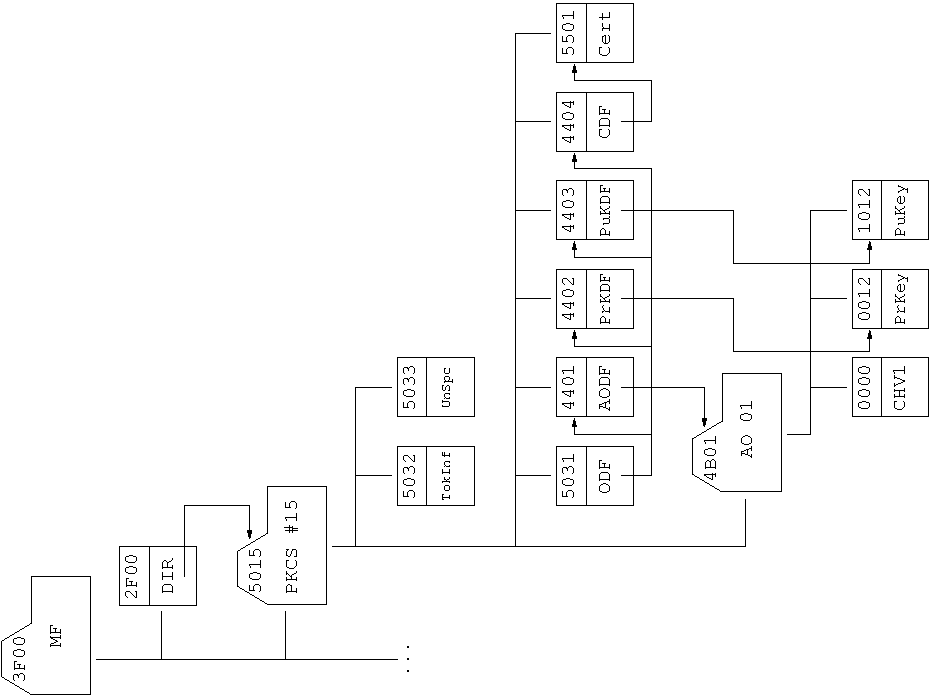
\includegraphics[angle=-90,scale=.6]{img/pkcs15fs.pdf}
	\caption{Przykładowa struktura aplikacji PKCS~\#15}
	\label{ppkcs15fs}
    \end{center}
\end{figure}

\begin{thm}
\label{thm}
Niech $x_1, x_2, x_3, \ldots$ będą dowolnymi zmiennymi o wartościach
należących do zbiorów $X_1, X_2, X_3, \ldots$.
\end{thm}

\begin{note}
Zdanie jest spełnione wyłącznie w dziedzinie $D_1$.
\end{note}

\begin{proof}[Dowód Twierdzenia \ref{thm}.]
Załóżmy, że twierdzenie \ref{thm} nie jest prawdziwe. Wtedy zachodzi:
\begin{equation}
G(t)=L\gamma!\,t^{-\gamma}+t^{-\delta}\eta(t) \qedhere
\end{equation}
\end{proof}

\section{Przykład trzeci}

W~ostatnim dziesięcioleciu, wraz z~silnym rozwojem aplikacji i~urządzeń
wykorzystujących algorytmy kryptograficzne, pojawiło się szereg problemów
związanych z~uniwersalnością zapisu danych wykorzystywanych podczas tych
operacji. Jedna z~amerykańskich firm, będąca liderem na rynku biznesowych
zastosowań kryptografii, postanowiła opracować własne formuły zapisu
informacji kryptograficznych. Brak dyskusji nad proponowanymi zaleceniami
(w przeciwieństwie do głosowania nad normami ISO/IEC) pozwolił na szybkie ogłoszenie
początkowych wersji dokumentów oraz ich wdrożenie. Pomysł przyjął się i~
dzięki temu powstały normy przemysłowe dotyczące kryptografii.

Firma {\bf RSA Data Security, Inc.}, bo o~niej mowa, zaproponowała szereg zaleceń
związanych z~interfejsem dla kryptografii z~kluczem publicznym. Znane są one pod
ogólną nazwą PKCS (ang. {\em Public Key Cryptography Standards}).
Wnioskując jedynie po ogólnym tytule można odnieść wrażenie, że zalecenia
objęły jedynie algorytmy asymetryczne (w których występuje para kluczy -
jawny, zwany publicznym oraz tajny, zwany prywatnym). Twórcy poruszyli
również tematykę związaną z~szerokim zastosowaniem tych algorytmów, dzięki
czemu zalecenia zawierają praktycznie wszystkie najważniejsze i~
najaktualniejsze informacje dotyczące praktycznych zastosowań kryptografii.

Lista dokumentów z~serii PKCS jest następująca:
\begin{itemize}
    \item PKCS \#1: {\em RSA Cryptography Standard} -- zawiera opis
    algorytmu RSA zarówno w~odniesieniu do podpisu cyfrowego jak i~
    kopert cyfrowych\footnote{dokumenty o~identyfikatorach \#2 i~\#4
    zostały połączone w~\#1}
    \item PKCS \#3: {\em Diffie-Hellman Key Agreement Standard} -- opisuje
    sposób implementacji algorytmu uzgadniania kluczy metodą
    Diffiego-Hellmana
    \item PKCS \#5: {\em Password-Based Cryptography Standard} -- zawiera
    opis metody bezpiecznej wymiany kluczy prywatnych
    \item PKCS \#6: {\em Extended-Certificate Syntax Standard} --
    opisuje budowę certyfikatów klucza publicznego X.509
    \item PKCS \#7: {\em Cryptographic Message Syntax Standard} -- jest to
    abstrakcyjny opis danych, które podlegają operacjom kryptograficznym
    \item PKCS \#8: {\em Private-Key Information Syntax Standard} --
    zawiera abstrakcyjny opis dotyczący składowania kluczy prywatnych (w
    formie jawnej i~zaszyfrowanej) wraz z~zestawem atrybutów
    \item PKCS \#9: {\em Selected Attribute Types} -- zawiera definicję
    atrybutów związanych z~certyfikatami, podpisami cyfrowymi i~kluczami
    prywatnymi
    \item PKCS \#10: {\em Certification Request Syntax Standard} --
    opisuje format żądania certyfikacyjnego
    \item PKCS~\#11: {\em Cryptographic Token Interface Standard} --
    opisuje abstrakcyjny interfejs programisty dla różnych typów urządzeń
    kryptograficznych
    \item PKCS \#12: {\em Personal Information Exchange Syntax
    Standard} -- zawiera opis formatu zapisu danych kryptograficznych przez
    aplikacje
    \item PKCS \#13: {\em Elliptic Curve Cryptography Standard} -- zawiera
    opis algorytmów opartych na krzywych eliptycznych
    \item PKCS \#14: {\em Pseudo Random Number Generation} -- zawiera
    opis algorytmów związanych z~generacją liczb
    pseudolosowych\footnote{aktualnie dokument ten jest opracowywany}
    \item PKCS~\#15: {\em Cryptographic Token Information Format
    Standard} -- opisuje sposób zapisu danych w~żetonach kryptograficznych
    (takich jak karty procesorowe)
\end{itemize}

Wszystkie publikacje dostępne są pod adresem internetowym
\url{http://www.rsasecurity.com/rsalabs/}.

\section{Przykład czwarty}

{\it Xfig}\footnote{\url{http://www.xfig.org/}}
i~{\it Dia}\footnote{\url{http://www.gnome.org/projects/dia/},
\url{http://dia-installer.sourceforge.net/}}
to aplikacje wspomagające tworzenie rysunków w~grafice wektorowej.
Pierwsza z~nich przeznaczona jest głownie do tworzenia obrazów
z~prostych elementów takich jak linie, prostokąty, okręgi, łuki.
{\it Dia}, wzorowane na {\it Visio} firmy {\it Microsoft}, posiada
wiele bibliotek graficznych i~jest najbardziej pomocne do
tworzenia skomplikowanych diagramów np. w~UML. Obie aplikacje obsługują
szeroki wachlarz formatów plików graficznych, co pozwala na wykorzystanie
rysunków stworzonych z~ich pomocą w~wielu programach służących do edycji
lub składu dokumentów.

Rysunek \ref{fig:xfig} obrazuje program {\it Xfig} podczas pracy nad jednym
z~rysunków wykorzystanych w~publikacji~\cite{bk:ipki}.
\begin{figure}[htb]
    \begin{center}
    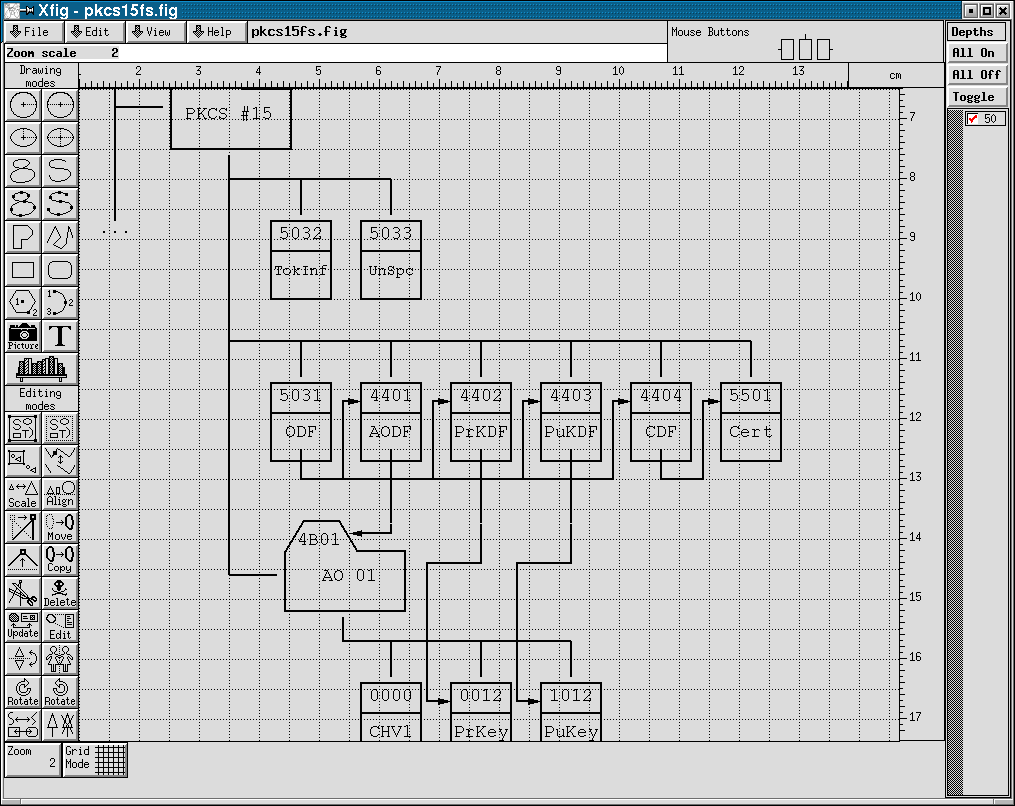
\includegraphics[angle=0,scale=.35]{img/xfig.png}
    \end{center}
    \caption{\em Xfig}
    \label{fig:xfig}
\end{figure}

\section{Przykład piąty}

Po utworzeniu pliku konfiguracyjnego można przystąpić do przygotowania
katalogów służących do przechowywania danych CA (zgodnie z~wcześniej
założonymi nazwami w~{\em openssl.cnf}). Tworzymy katalog {\em ca}, a~w nim
katalogi {\em certs}, {\em crl}, {\em private}, {\em newcerts} oraz pliki
{\em serial.txt} (z wpisem 01) i~{\em index.txt}. Plik {\em openssl.cnf} należy
umieścić na tym samym poziomie co katalog {\em ca}. Oczywiście możliwe jest
zupełnie inne zorganizowanie sposobu przechowywania danych w~CA, jednak
musi ono odpowiadać wcześniej przyjętym założeniom w pliku konfiguracyjnym.

Następnym krokiem przy tworzeniu CA jest wygenerowanie pary kluczy oraz
autocertyfikatu (w przypadku, gdy certyfikat dla centrum nie będzie
poświadczany przez inne centrum certyfikacji) dla centrum certyfikacji.

\begin{verbatim}
# generacja klucza prywatnego RSA o długości 4096 bitów
# do pliku cakey.pem (klucz w formie jawnej)
openssl genrsa -out ca/private/cakey.pem 4096 -config openssl.cnf

# utworzenie autocertyfikatu centrum (cacert.pem) o strukturze
# X.509 i formacie PEM dla klucza jawnego związanego z kluczem
# tajnym cakey.pem
openssl req -new -x509 -days 1825 -key ca/private/cakey.pem -out
    ca/cacert.pem -config openssl.cnf
\end{verbatim}

Po tych operacjach CA jest gotowe do pracy.

\section{Przykład szósty}

Oto przykładowy wydruk:
\begin{lstlisting}[language=Java,style=outcode,caption=Przykładowy wydruk]
import a.b.c;

// komentarz

/*
 * Komentarz...
 */
public class A
{
	int A;
	int B; // zmienna

	A()
	{
		A=1;
		/* to jest komentarz */
	}

	public void metodaA(int i)
	{
		for (int a=i; a<100; ++a)
		{
			short sw=(short)a;
			// ...
		}
	}
}
\end{lstlisting}

A oto wydruk wpleciony w tekst\dots
\begin{lstlisting}[language=C,style=incode]
/* ta funkcja oblicza a+b */
int sum(int a, int b)
{
	int suma=0;

	suma=a+b;

	return suma;
}
\end{lstlisting}
\dots i tekst za kodem.

% \lstinputlisting[language=Java,style=incode]{nazwa pliku}

% ex: set tabstop=4 shiftwidth=4 softtabstop=4 noexpandtab fileformat=unix filetype=tex spelllang=pl,en spell:
